\chapter{Problem Analysis}
This chapter examines existing literature concerning source localisation from EEG measurements. At first a motivation for the problem is given, considering especially the application within the hearing aid industry. Further, the state of the art methods are presented followed by a description of the contribution proposed in this thesis. 

\section{Motivation}
(Hvad er EEG)\\
EEG recordings or measurements are used within medicine as an imaging technique measuring electric signals on the scalp, caused by brain activity. \\
\\
The brain consist of an enormous amounts of cells, called neurons. These neurons are mutually connected in neural nets and when a neuron is activated, for instance by some physical stimuli, local current flows are produced\cite{fundamentalEEG}. As such the neurons are somehow communicating(?). \\
\\
The EEG measurements are provided by a varies number of metal electrodes referred to as sensors, placed on the scalp of a human reading electrical signals which are massively amplified and displayed on the computer as a sum of sinusoidal waves relative to time.\\
It takes a large amount of active neurons to generate an electrical signal that is recordable on the scalp as the current then have to penetrate the skull, skin and several other thin layers.  \\
From this it is clear that the measurements from a single sensor do not correspond to the activity of a single neuron in the brain, but rather a collection of many activities. Here the same neuron activities can be measured by two or more sensors. Furthermore, interfering signals can occur resulting from physical movement of e.g. eyes and jawbone\cite{fundamentalEEG}.\\
\\
The waves resulting from EEG have been classified into four groups according to the dominant frequency. The delta wave ($0.5-4$ Hz) is observed from infants and sleeping adults, the Theta wave ($4-8$ Hz) is observed from children and sleeping adults, the alpha wave ($8-13$ Hz) is the most extensively studied brain rhythm, which is induced by an adult laying down with closed eyes. Lastly the beta wave ($13-30$ Hz) is considered the normal brain rhythm for normal adults, associated with active thinking, active attention or solving concrete problems\cite[p. 11]{EEGsignalprocessing}. An example of EEG measurement within the four categories are illustrated by figure \ref{fig:EEG_example}.        
\begin{figure}[h]
    \centering
    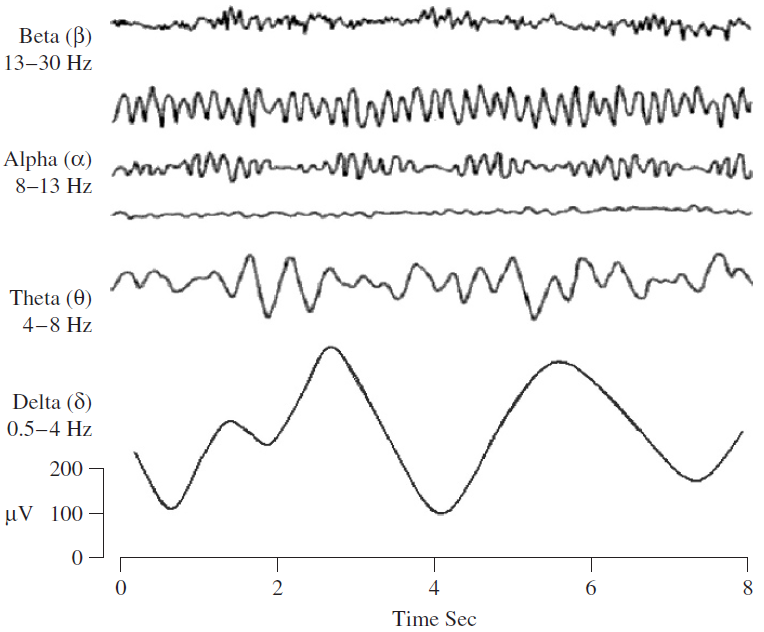
\includegraphics[scale=0.65]{figurs/EEG_example.png}
    \caption{Example of time dependent EEG measurements within the four defined categories alpha, beta, theta and delta. Image source: \cite{EEGsignalprocessing}}
    \label{fig:EEG_example}
\end{figure}
Evoked potential 


(Hvad bruges det til)\\
EEG is widely used within medicine and research of the cognitive processes in the brain. Diagnosis and Management of neurological disorders such as epilepsy is one example. \\   
A great advantage of EEG is the speed. Neural activity can be measured within fractions of a second after a stimuli has been provided. When a person is exposed to certain stimuli, e.g. visual or audible, the measured activity is said to result from evoked potential.   
 

(Hvad er problemet, localisation)\\

(Anvendelse i praksis)

evt. lave subsections her..

\section{Related Work and Our Contribution } 
indhold
\\
\\
nb. husk at dette kapitel skal vise et helt system og hvorhenne i det system vi kigger nærmere og kommer ind med vores bidrag. Det skal gøres klar hvilke områder vi vælger at ligge vores kræfter i.  





 
